% Options for packages loaded elsewhere
\PassOptionsToPackage{unicode}{hyperref}
\PassOptionsToPackage{hyphens}{url}
%
\documentclass[
]{article}
\usepackage{amsmath,amssymb}
\usepackage{lmodern}
\usepackage{iftex}
\ifPDFTeX
  \usepackage[T1]{fontenc}
  \usepackage[utf8]{inputenc}
  \usepackage{textcomp} % provide euro and other symbols
\else % if luatex or xetex
  \usepackage{unicode-math}
  \defaultfontfeatures{Scale=MatchLowercase}
  \defaultfontfeatures[\rmfamily]{Ligatures=TeX,Scale=1}
\fi
% Use upquote if available, for straight quotes in verbatim environments
\IfFileExists{upquote.sty}{\usepackage{upquote}}{}
\IfFileExists{microtype.sty}{% use microtype if available
  \usepackage[]{microtype}
  \UseMicrotypeSet[protrusion]{basicmath} % disable protrusion for tt fonts
}{}
\makeatletter
\@ifundefined{KOMAClassName}{% if non-KOMA class
  \IfFileExists{parskip.sty}{%
    \usepackage{parskip}
  }{% else
    \setlength{\parindent}{0pt}
    \setlength{\parskip}{6pt plus 2pt minus 1pt}}
}{% if KOMA class
  \KOMAoptions{parskip=half}}
\makeatother
\usepackage{xcolor}
\IfFileExists{xurl.sty}{\usepackage{xurl}}{} % add URL line breaks if available
\IfFileExists{bookmark.sty}{\usepackage{bookmark}}{\usepackage{hyperref}}
\hypersetup{
  pdftitle={Assignment 1},
  pdfauthor={630516am and 590049bm},
  hidelinks,
  pdfcreator={LaTeX via pandoc}}
\urlstyle{same} % disable monospaced font for URLs
\usepackage[margin=1in]{geometry}
\usepackage{color}
\usepackage{fancyvrb}
\newcommand{\VerbBar}{|}
\newcommand{\VERB}{\Verb[commandchars=\\\{\}]}
\DefineVerbatimEnvironment{Highlighting}{Verbatim}{commandchars=\\\{\}}
% Add ',fontsize=\small' for more characters per line
\usepackage{framed}
\definecolor{shadecolor}{RGB}{248,248,248}
\newenvironment{Shaded}{\begin{snugshade}}{\end{snugshade}}
\newcommand{\AlertTok}[1]{\textcolor[rgb]{0.94,0.16,0.16}{#1}}
\newcommand{\AnnotationTok}[1]{\textcolor[rgb]{0.56,0.35,0.01}{\textbf{\textit{#1}}}}
\newcommand{\AttributeTok}[1]{\textcolor[rgb]{0.77,0.63,0.00}{#1}}
\newcommand{\BaseNTok}[1]{\textcolor[rgb]{0.00,0.00,0.81}{#1}}
\newcommand{\BuiltInTok}[1]{#1}
\newcommand{\CharTok}[1]{\textcolor[rgb]{0.31,0.60,0.02}{#1}}
\newcommand{\CommentTok}[1]{\textcolor[rgb]{0.56,0.35,0.01}{\textit{#1}}}
\newcommand{\CommentVarTok}[1]{\textcolor[rgb]{0.56,0.35,0.01}{\textbf{\textit{#1}}}}
\newcommand{\ConstantTok}[1]{\textcolor[rgb]{0.00,0.00,0.00}{#1}}
\newcommand{\ControlFlowTok}[1]{\textcolor[rgb]{0.13,0.29,0.53}{\textbf{#1}}}
\newcommand{\DataTypeTok}[1]{\textcolor[rgb]{0.13,0.29,0.53}{#1}}
\newcommand{\DecValTok}[1]{\textcolor[rgb]{0.00,0.00,0.81}{#1}}
\newcommand{\DocumentationTok}[1]{\textcolor[rgb]{0.56,0.35,0.01}{\textbf{\textit{#1}}}}
\newcommand{\ErrorTok}[1]{\textcolor[rgb]{0.64,0.00,0.00}{\textbf{#1}}}
\newcommand{\ExtensionTok}[1]{#1}
\newcommand{\FloatTok}[1]{\textcolor[rgb]{0.00,0.00,0.81}{#1}}
\newcommand{\FunctionTok}[1]{\textcolor[rgb]{0.00,0.00,0.00}{#1}}
\newcommand{\ImportTok}[1]{#1}
\newcommand{\InformationTok}[1]{\textcolor[rgb]{0.56,0.35,0.01}{\textbf{\textit{#1}}}}
\newcommand{\KeywordTok}[1]{\textcolor[rgb]{0.13,0.29,0.53}{\textbf{#1}}}
\newcommand{\NormalTok}[1]{#1}
\newcommand{\OperatorTok}[1]{\textcolor[rgb]{0.81,0.36,0.00}{\textbf{#1}}}
\newcommand{\OtherTok}[1]{\textcolor[rgb]{0.56,0.35,0.01}{#1}}
\newcommand{\PreprocessorTok}[1]{\textcolor[rgb]{0.56,0.35,0.01}{\textit{#1}}}
\newcommand{\RegionMarkerTok}[1]{#1}
\newcommand{\SpecialCharTok}[1]{\textcolor[rgb]{0.00,0.00,0.00}{#1}}
\newcommand{\SpecialStringTok}[1]{\textcolor[rgb]{0.31,0.60,0.02}{#1}}
\newcommand{\StringTok}[1]{\textcolor[rgb]{0.31,0.60,0.02}{#1}}
\newcommand{\VariableTok}[1]{\textcolor[rgb]{0.00,0.00,0.00}{#1}}
\newcommand{\VerbatimStringTok}[1]{\textcolor[rgb]{0.31,0.60,0.02}{#1}}
\newcommand{\WarningTok}[1]{\textcolor[rgb]{0.56,0.35,0.01}{\textbf{\textit{#1}}}}
\usepackage{graphicx}
\makeatletter
\def\maxwidth{\ifdim\Gin@nat@width>\linewidth\linewidth\else\Gin@nat@width\fi}
\def\maxheight{\ifdim\Gin@nat@height>\textheight\textheight\else\Gin@nat@height\fi}
\makeatother
% Scale images if necessary, so that they will not overflow the page
% margins by default, and it is still possible to overwrite the defaults
% using explicit options in \includegraphics[width, height, ...]{}
\setkeys{Gin}{width=\maxwidth,height=\maxheight,keepaspectratio}
% Set default figure placement to htbp
\makeatletter
\def\fps@figure{htbp}
\makeatother
\setlength{\emergencystretch}{3em} % prevent overfull lines
\providecommand{\tightlist}{%
  \setlength{\itemsep}{0pt}\setlength{\parskip}{0pt}}
\setcounter{secnumdepth}{-\maxdimen} % remove section numbering
\usepackage{booktabs}
\usepackage{siunitx}
\newcolumntype{d}{S[input-symbols = ()]}
\usepackage{longtable}
\usepackage{array}
\usepackage{multirow}
\usepackage{wrapfig}
\usepackage{float}
\usepackage{colortbl}
\usepackage{pdflscape}
\usepackage{tabu}
\usepackage{threeparttable}
\usepackage{threeparttablex}
\usepackage[normalem]{ulem}
\usepackage{makecell}
\usepackage{xcolor}
\ifLuaTeX
  \usepackage{selnolig}  % disable illegal ligatures
\fi

\title{Assignment 1}
\author{630516am and 590049bm}
\date{15/3/2021}

\begin{document}
\maketitle

\hypertarget{assignment-1}{%
\subsection{Assignment 1}\label{assignment-1}}

At the beginning of the code,set the random seed to 810 using
set.seed(). Failure to do so will be penalised.

\small

\begin{Shaded}
\begin{Highlighting}[]
\FunctionTok{set.seed}\NormalTok{(}\DecValTok{810}\NormalTok{)}
\end{Highlighting}
\end{Shaded}

\normalsize

\begin{enumerate}
\def\labelenumi{\alph{enumi}.}
\tightlist
\item
  Simulate 100,000 observations from the DGP
\end{enumerate}

\small

\begin{Shaded}
\begin{Highlighting}[]
\NormalTok{x }\OtherTok{\textless{}{-}} \FunctionTok{rnorm}\NormalTok{(}\DecValTok{100000}\NormalTok{, }\AttributeTok{mean =} \DecValTok{6}\NormalTok{, }\AttributeTok{sd =} \FunctionTok{sqrt}\NormalTok{(}\DecValTok{3}\NormalTok{))}
\NormalTok{alpha }\OtherTok{\textless{}{-}} \DecValTok{5}
\NormalTok{e }\OtherTok{\textless{}{-}} \FunctionTok{rnorm}\NormalTok{(}\DecValTok{100000}\NormalTok{, }\DecValTok{0}\NormalTok{, }\DecValTok{1}\NormalTok{)}
\NormalTok{y }\OtherTok{\textless{}{-}}\NormalTok{ alpha }\SpecialCharTok{+} \FloatTok{0.3}\SpecialCharTok{*}\NormalTok{x }\SpecialCharTok{+} \FloatTok{0.1}\SpecialCharTok{*}\NormalTok{x}\SpecialCharTok{\^{}}\DecValTok{2} \SpecialCharTok{+}\NormalTok{ e}
\NormalTok{dataset }\OtherTok{\textless{}{-}} \FunctionTok{data.frame}\NormalTok{(}\AttributeTok{x =}\NormalTok{ x, }\AttributeTok{x\_sq =}\NormalTok{ x}\SpecialCharTok{\^{}}\DecValTok{2}\NormalTok{, }\AttributeTok{y =}\NormalTok{ y)}
\end{Highlighting}
\end{Shaded}

\normalsize

\small

\begin{Shaded}
\begin{Highlighting}[]
\NormalTok{p1 }\OtherTok{\textless{}{-}}\NormalTok{ dataset }\SpecialCharTok{\%\textgreater{}\%}
    \FunctionTok{ggplot}\NormalTok{(}\FunctionTok{aes}\NormalTok{(}\AttributeTok{x =}\NormalTok{ x)) }\SpecialCharTok{+} \FunctionTok{geom\_histogram}\NormalTok{(}\AttributeTok{bins =} \DecValTok{50}\NormalTok{)}
\NormalTok{p2 }\OtherTok{\textless{}{-}}\NormalTok{ dataset }\SpecialCharTok{\%\textgreater{}\%}
    \FunctionTok{ggplot}\NormalTok{(}\FunctionTok{aes}\NormalTok{(}\AttributeTok{x =}\NormalTok{ x\_sq)) }\SpecialCharTok{+} \FunctionTok{geom\_histogram}\NormalTok{(}\AttributeTok{bins =} \DecValTok{50}\NormalTok{)}
\NormalTok{p3 }\OtherTok{\textless{}{-}}\NormalTok{ dataset }\SpecialCharTok{\%\textgreater{}\%}
    \FunctionTok{ggplot}\NormalTok{(}\FunctionTok{aes}\NormalTok{(}\AttributeTok{x =}\NormalTok{ y)) }\SpecialCharTok{+} \FunctionTok{geom\_histogram}\NormalTok{(}\AttributeTok{bins =} \DecValTok{50}\NormalTok{)}
\NormalTok{p4 }\OtherTok{\textless{}{-}}\NormalTok{ dataset }\SpecialCharTok{\%\textgreater{}\%}
    \FunctionTok{ggplot}\NormalTok{(}\FunctionTok{aes}\NormalTok{(}\AttributeTok{x =}\NormalTok{ x, }\AttributeTok{y =}\NormalTok{ y)) }\SpecialCharTok{+} \FunctionTok{geom\_point}\NormalTok{()}
\NormalTok{cowplot}\SpecialCharTok{::}\FunctionTok{plot\_grid}\NormalTok{(p1, p2, p3, p4, }\AttributeTok{nrow =} \DecValTok{2}\NormalTok{, }\AttributeTok{ncol =} \DecValTok{2}\NormalTok{)}
\end{Highlighting}
\end{Shaded}

\begin{center}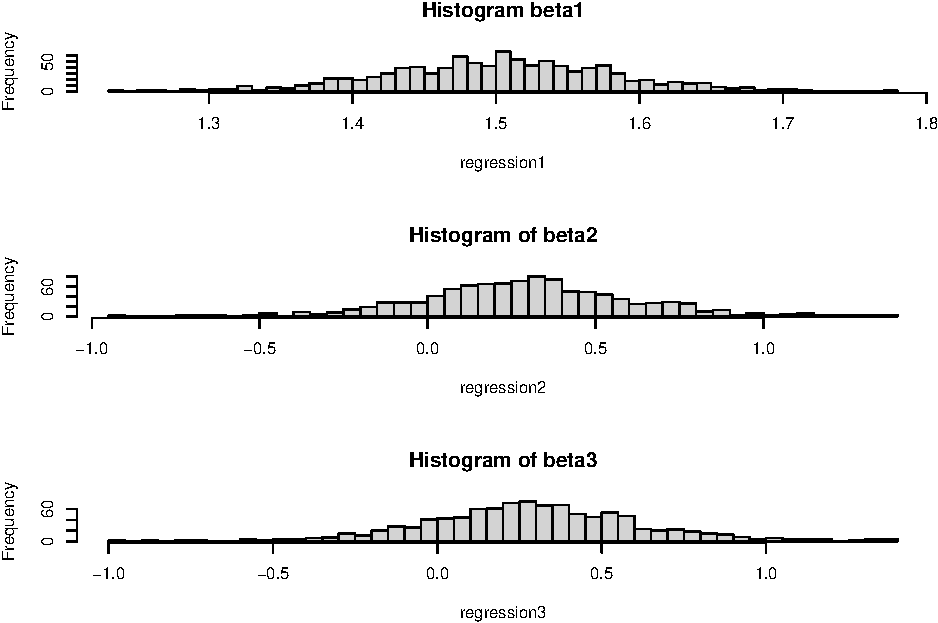
\includegraphics[width=250pt,height=200pt]{assignment_1_files/figure-latex/unnamed-chunk-3-1} \end{center}

\normalsize

\begin{enumerate}
\def\labelenumi{\alph{enumi}.}
\setcounter{enumi}{1}
\tightlist
\item
  Break the data into 1000 datasets of 100 observations sequentially
  (i.e.~dataset 1 comprises observations 1-100 from your simulation,
  dataset 2 comprises observations 101-200 and so on
\end{enumerate}

\small

\begin{Shaded}
\begin{Highlighting}[]
\NormalTok{hundred }\OtherTok{\textless{}{-}}\NormalTok{ dataset }\SpecialCharTok{\%\textgreater{}\%} 
   \FunctionTok{group\_by}\NormalTok{((}\FunctionTok{row\_number}\NormalTok{()}\SpecialCharTok{{-}}\DecValTok{1}\NormalTok{) }\SpecialCharTok{\%/\%}\NormalTok{ (}\FunctionTok{n}\NormalTok{()}\SpecialCharTok{/}\DecValTok{1000}\NormalTok{)) }\SpecialCharTok{\%\textgreater{}\%}
\NormalTok{   nest }\SpecialCharTok{\%\textgreater{}\%} \FunctionTok{pull}\NormalTok{(data)}
\end{Highlighting}
\end{Shaded}

\normalsize

\small

\begin{Shaded}
\begin{Highlighting}[]
\NormalTok{beta1 }\OtherTok{\textless{}{-}} \FunctionTok{map\_dbl}\NormalTok{(hundred, }\SpecialCharTok{\textasciitilde{}} \FunctionTok{lm}\NormalTok{(}\AttributeTok{data =}\NormalTok{ .x, }\AttributeTok{formula =}\NormalTok{ y }\SpecialCharTok{\textasciitilde{}}\NormalTok{ x }\SpecialCharTok{+}\NormalTok{ x\_sq) }\SpecialCharTok{\%\textgreater{}\%}
\NormalTok{    .}\SpecialCharTok{$}\NormalTok{coefficients }\SpecialCharTok{\%\textgreater{}\%}
\NormalTok{    .[}\DecValTok{2}\NormalTok{])}
\NormalTok{se1 }\OtherTok{\textless{}{-}} \FunctionTok{map\_dbl}\NormalTok{(hundred, }\SpecialCharTok{\textasciitilde{}} \FunctionTok{lm}\NormalTok{(}\AttributeTok{data =}\NormalTok{ .x, }\AttributeTok{formula =}\NormalTok{ y }\SpecialCharTok{\textasciitilde{}}\NormalTok{ x }\SpecialCharTok{+}\NormalTok{ x\_sq) }\SpecialCharTok{\%\textgreater{}\%}
                  \FunctionTok{summary}\NormalTok{() }\SpecialCharTok{\%\textgreater{}\%}
\NormalTok{                  .}\SpecialCharTok{$}\NormalTok{coefficients }\SpecialCharTok{\%\textgreater{}\%}
\NormalTok{                  .[}\DecValTok{2}\NormalTok{,}\DecValTok{2}\NormalTok{])}
\NormalTok{p1\_een }\OtherTok{\textless{}{-}} \FunctionTok{data.frame}\NormalTok{(}\AttributeTok{b1 =}\NormalTok{ beta1, }\AttributeTok{se1 =}\NormalTok{ se1) }\SpecialCharTok{\%\textgreater{}\%}
    \FunctionTok{ggplot}\NormalTok{(}\FunctionTok{aes}\NormalTok{(}\AttributeTok{x =}\NormalTok{ b1)) }\SpecialCharTok{+} \FunctionTok{geom\_histogram}\NormalTok{()}
\NormalTok{p2\_een }\OtherTok{\textless{}{-}} \FunctionTok{data.frame}\NormalTok{(}\AttributeTok{b1 =}\NormalTok{ beta1, }\AttributeTok{se1 =}\NormalTok{ se1) }\SpecialCharTok{\%\textgreater{}\%}
    \FunctionTok{ggplot}\NormalTok{(}\FunctionTok{aes}\NormalTok{(}\AttributeTok{x =}\NormalTok{ se1)) }\SpecialCharTok{+} \FunctionTok{geom\_histogram}\NormalTok{()}
\NormalTok{cowplot}\SpecialCharTok{::}\FunctionTok{plot\_grid}\NormalTok{(p1\_een, p2\_een)}
\end{Highlighting}
\end{Shaded}

\begin{center}\includegraphics[width=250pt,height=200pt]{assignment_1_files/figure-latex/unnamed-chunk-5-1} \end{center}

\normalsize

\small

\begin{Shaded}
\begin{Highlighting}[]
\NormalTok{beta\_omv }\OtherTok{\textless{}{-}} \FunctionTok{map\_dbl}\NormalTok{(hundred, }\SpecialCharTok{\textasciitilde{}} \FunctionTok{lm}\NormalTok{(}\AttributeTok{data =}\NormalTok{ .x, }\AttributeTok{formula =}\NormalTok{ y }\SpecialCharTok{\textasciitilde{}}\NormalTok{ x) }\SpecialCharTok{\%\textgreater{}\%}
\NormalTok{    .}\SpecialCharTok{$}\NormalTok{coefficients }\SpecialCharTok{\%\textgreater{}\%}
\NormalTok{    .[}\DecValTok{2}\NormalTok{])}
\NormalTok{se\_omv }\OtherTok{\textless{}{-}} \FunctionTok{map\_dbl}\NormalTok{(hundred, }\SpecialCharTok{\textasciitilde{}} \FunctionTok{lm}\NormalTok{(}\AttributeTok{data =}\NormalTok{ .x, }\AttributeTok{formula =}\NormalTok{ y }\SpecialCharTok{\textasciitilde{}}\NormalTok{ x) }\SpecialCharTok{\%\textgreater{}\%}
                  \FunctionTok{summary}\NormalTok{() }\SpecialCharTok{\%\textgreater{}\%}
\NormalTok{                  .}\SpecialCharTok{$}\NormalTok{coefficients }\SpecialCharTok{\%\textgreater{}\%}
\NormalTok{                  .[}\DecValTok{2}\NormalTok{,}\DecValTok{2}\NormalTok{])}
\NormalTok{p1\_omv }\OtherTok{\textless{}{-}} \FunctionTok{data.frame}\NormalTok{(}\AttributeTok{b1 =}\NormalTok{ beta\_omv, }\AttributeTok{se1 =}\NormalTok{ se\_omv) }\SpecialCharTok{\%\textgreater{}\%}
    \FunctionTok{ggplot}\NormalTok{(}\FunctionTok{aes}\NormalTok{(}\AttributeTok{x =}\NormalTok{ b1)) }\SpecialCharTok{+} \FunctionTok{geom\_histogram}\NormalTok{()}
\NormalTok{p2\_omv }\OtherTok{\textless{}{-}} \FunctionTok{data.frame}\NormalTok{(}\AttributeTok{b1 =}\NormalTok{ beta\_omv, }\AttributeTok{se1 =}\NormalTok{ se\_omv) }\SpecialCharTok{\%\textgreater{}\%}
    \FunctionTok{ggplot}\NormalTok{(}\FunctionTok{aes}\NormalTok{(}\AttributeTok{x =}\NormalTok{ se1)) }\SpecialCharTok{+} \FunctionTok{geom\_histogram}\NormalTok{()}
\NormalTok{cowplot}\SpecialCharTok{::}\FunctionTok{plot\_grid}\NormalTok{(p1\_omv, p2\_omv)}
\end{Highlighting}
\end{Shaded}

\begin{center}\includegraphics[width=250pt,height=200pt]{assignment_1_files/figure-latex/unnamed-chunk-6-1} \end{center}

\normalsize

We see that the coefficients from the fully specified model (without
omitted variable biased) are normally distributed around the true
coefficient value from the DGP, whereas the coefficient in the wrongly
specified model is noisy distributed around a wrong value.

\begin{enumerate}
\def\labelenumi{\alph{enumi}.}
\setcounter{enumi}{2}
\tightlist
\item
  Imagine we had instead generated \(X_i = c\) for all \(x_i\) and tried
  to perform our simulation above. This would fail because we would
  violate one of the necessary conditions for computing the least
  squares estimator. Which one, and how?
\end{enumerate}

We would violate assumption 1:

\[
\sum_{i=1}^{N} (x_i - \bar{x})^2 > 0 
\] as the sum of the square of the difference between Xi and X bar would
be zero if \(X_i = c\). Xi = c would also mean that X is not full rank
and therefore not invertible. Hence, we could not calculate the least
squares estimator.

\begin{enumerate}
\def\labelenumi{\alph{enumi}.}
\setcounter{enumi}{3}
\tightlist
\item
  Simulate another dataset as in a), but with 1,000,000 observations.
  Repeat part b), but now using 1000 observations per model. Only fit
  the equation \(Y_i = \alpha + \beta_1 X_i + \beta_2 X_i^2 + \epsilon\)
  this time. Plot the histograms of the estimate of \(\beta_1\) and
  \(se(\beta_1)\) and compare them to the estimates from the same model
  in (b). What happens to the distribution of the coefficient estimates
  and standard errors when we increase the sample size per model?
\end{enumerate}

\small

\begin{Shaded}
\begin{Highlighting}[]
\NormalTok{x2 }\OtherTok{\textless{}{-}} \FunctionTok{rnorm}\NormalTok{(}\DecValTok{1000000}\NormalTok{, }\AttributeTok{mean =} \DecValTok{6}\NormalTok{, }\AttributeTok{sd =} \FunctionTok{sqrt}\NormalTok{(}\DecValTok{3}\NormalTok{))}
\NormalTok{alpha2 }\OtherTok{\textless{}{-}} \DecValTok{5}
\NormalTok{e2 }\OtherTok{\textless{}{-}} \FunctionTok{rnorm}\NormalTok{(}\DecValTok{1000000}\NormalTok{, }\DecValTok{0}\NormalTok{, }\DecValTok{1}\NormalTok{)}
\NormalTok{y2 }\OtherTok{\textless{}{-}}\NormalTok{ alpha2 }\SpecialCharTok{+} \FloatTok{0.3}\SpecialCharTok{*}\NormalTok{x2 }\SpecialCharTok{+} \FloatTok{0.1}\SpecialCharTok{*}\NormalTok{x2}\SpecialCharTok{\^{}}\DecValTok{2} \SpecialCharTok{+}\NormalTok{ e2}
\NormalTok{dataset2 }\OtherTok{\textless{}{-}} \FunctionTok{data.frame}\NormalTok{(}\AttributeTok{x =}\NormalTok{ x2, }\AttributeTok{x\_sq =}\NormalTok{ x2}\SpecialCharTok{\^{}}\DecValTok{2}\NormalTok{, }\AttributeTok{y =}\NormalTok{ y2)}
\end{Highlighting}
\end{Shaded}

\normalsize

\small

\begin{Shaded}
\begin{Highlighting}[]
\NormalTok{thousand }\OtherTok{\textless{}{-}}\NormalTok{ dataset2 }\SpecialCharTok{\%\textgreater{}\%} 
   \FunctionTok{group\_by}\NormalTok{((}\FunctionTok{row\_number}\NormalTok{()}\SpecialCharTok{{-}}\DecValTok{1}\NormalTok{) }\SpecialCharTok{\%/\%}\NormalTok{ (}\FunctionTok{n}\NormalTok{()}\SpecialCharTok{/}\DecValTok{1000}\NormalTok{)) }\SpecialCharTok{\%\textgreater{}\%}
\NormalTok{   nest }\SpecialCharTok{\%\textgreater{}\%} \FunctionTok{pull}\NormalTok{(data)}
\end{Highlighting}
\end{Shaded}

\normalsize

\small

\begin{Shaded}
\begin{Highlighting}[]
\NormalTok{beta\_ef }\OtherTok{\textless{}{-}} \FunctionTok{map\_dbl}\NormalTok{(thousand, }\SpecialCharTok{\textasciitilde{}} \FunctionTok{lm}\NormalTok{(}\AttributeTok{data =}\NormalTok{ .x, }\AttributeTok{formula =}\NormalTok{ y }\SpecialCharTok{\textasciitilde{}}\NormalTok{ x }\SpecialCharTok{+}\NormalTok{ x\_sq) }\SpecialCharTok{\%\textgreater{}\%}
\NormalTok{    .}\SpecialCharTok{$}\NormalTok{coefficients }\SpecialCharTok{\%\textgreater{}\%}
\NormalTok{    .[}\DecValTok{2}\NormalTok{])}
\NormalTok{se\_ef }\OtherTok{\textless{}{-}} \FunctionTok{map\_dbl}\NormalTok{(thousand, }\SpecialCharTok{\textasciitilde{}} \FunctionTok{lm}\NormalTok{(}\AttributeTok{data =}\NormalTok{ .x, }\AttributeTok{formula =}\NormalTok{ y }\SpecialCharTok{\textasciitilde{}}\NormalTok{ x }\SpecialCharTok{+}\NormalTok{ x\_sq) }\SpecialCharTok{\%\textgreater{}\%}
                  \FunctionTok{summary}\NormalTok{() }\SpecialCharTok{\%\textgreater{}\%}
\NormalTok{                  .}\SpecialCharTok{$}\NormalTok{coefficients }\SpecialCharTok{\%\textgreater{}\%}
\NormalTok{                  .[}\DecValTok{2}\NormalTok{,}\DecValTok{2}\NormalTok{])}
\NormalTok{p1\_ef }\OtherTok{\textless{}{-}} \FunctionTok{data.frame}\NormalTok{(}\AttributeTok{b1 =}\NormalTok{ beta\_ef, }\AttributeTok{se1 =}\NormalTok{ se\_ef) }\SpecialCharTok{\%\textgreater{}\%}
    \FunctionTok{ggplot}\NormalTok{(}\FunctionTok{aes}\NormalTok{(}\AttributeTok{x =}\NormalTok{ b1)) }\SpecialCharTok{+} \FunctionTok{geom\_histogram}\NormalTok{()}
\NormalTok{p2\_ef }\OtherTok{\textless{}{-}} \FunctionTok{data.frame}\NormalTok{(}\AttributeTok{b1 =}\NormalTok{ beta\_ef, }\AttributeTok{se1 =}\NormalTok{ se\_ef) }\SpecialCharTok{\%\textgreater{}\%}
    \FunctionTok{ggplot}\NormalTok{(}\FunctionTok{aes}\NormalTok{(}\AttributeTok{x =}\NormalTok{ se1)) }\SpecialCharTok{+} \FunctionTok{geom\_histogram}\NormalTok{()}
\NormalTok{cowplot}\SpecialCharTok{::}\FunctionTok{plot\_grid}\NormalTok{(p1\_ef, p2\_ef)}
\end{Highlighting}
\end{Shaded}

\begin{center}\includegraphics[width=250pt,height=200pt]{assignment_1_files/figure-latex/unnamed-chunk-9-1} \end{center}

\normalsize Comparing this histogram to thr histogram from b), we can
see that the mean stays approximately the same. However, the spread and
therefore the variance of the estimate from d) is smaller than from the
estimate of b). This makes sense, as with an increasing number of
observations the variance of the estimate decreases. The same can be
observed with the standard error of the estimate. The mean stays
approximately the same but the variance of the standard error decreases.

\begin{enumerate}
\def\labelenumi{\alph{enumi}.}
\setcounter{enumi}{4}
\tightlist
\item
  Now, generate a new variable \(C_i\) that is correlated with \(X_i\).
  Do this by creating a vector of observations drawn from N(1,2) and
  adding them to \(X_i\). Add \(C_i\) the dataset from the previous
  questions (i.e with 100,000 observations total).
\end{enumerate}

\small

\begin{Shaded}
\begin{Highlighting}[]
\NormalTok{c }\OtherTok{\textless{}{-}} \FunctionTok{rnorm}\NormalTok{(}\DecValTok{100000}\NormalTok{, }\AttributeTok{mean =} \DecValTok{1}\NormalTok{, }\AttributeTok{sd =} \FunctionTok{sqrt}\NormalTok{(}\DecValTok{2}\NormalTok{)) }\SpecialCharTok{+}\NormalTok{ x}
\NormalTok{dataset }\OtherTok{\textless{}{-}} \FunctionTok{data.frame}\NormalTok{(}\AttributeTok{x =}\NormalTok{ x, }\AttributeTok{x\_sq =}\NormalTok{ x}\SpecialCharTok{\^{}}\DecValTok{2}\NormalTok{, }\AttributeTok{y =}\NormalTok{ y, }\AttributeTok{c =}\NormalTok{ c)}
\NormalTok{hundred }\OtherTok{\textless{}{-}}\NormalTok{ dataset }\SpecialCharTok{\%\textgreater{}\%} 
   \FunctionTok{group\_by}\NormalTok{((}\FunctionTok{row\_number}\NormalTok{()}\SpecialCharTok{{-}}\DecValTok{1}\NormalTok{) }\SpecialCharTok{\%/\%}\NormalTok{ (}\FunctionTok{n}\NormalTok{()}\SpecialCharTok{/}\DecValTok{1000}\NormalTok{)) }\SpecialCharTok{\%\textgreater{}\%}
\NormalTok{   nest }\SpecialCharTok{\%\textgreater{}\%} \FunctionTok{pull}\NormalTok{(data)}
\NormalTok{beta\_twee }\OtherTok{\textless{}{-}} \FunctionTok{map\_dbl}\NormalTok{(hundred, }\SpecialCharTok{\textasciitilde{}} \FunctionTok{lm}\NormalTok{(}\AttributeTok{data =}\NormalTok{ .x, }\AttributeTok{formula =}\NormalTok{ y }\SpecialCharTok{\textasciitilde{}}\NormalTok{ x }\SpecialCharTok{+}\NormalTok{ x\_sq }\SpecialCharTok{+}\NormalTok{ c) }\SpecialCharTok{\%\textgreater{}\%}
\NormalTok{    .}\SpecialCharTok{$}\NormalTok{coefficients }\SpecialCharTok{\%\textgreater{}\%}
\NormalTok{    .[}\DecValTok{2}\NormalTok{])}
\NormalTok{se\_twee }\OtherTok{\textless{}{-}} \FunctionTok{map\_dbl}\NormalTok{(hundred, }\SpecialCharTok{\textasciitilde{}} \FunctionTok{lm}\NormalTok{(}\AttributeTok{data =}\NormalTok{ .x, }\AttributeTok{formula =}\NormalTok{ y }\SpecialCharTok{\textasciitilde{}}\NormalTok{ x }\SpecialCharTok{+}\NormalTok{ x\_sq }\SpecialCharTok{+}\NormalTok{ c) }\SpecialCharTok{\%\textgreater{}\%}
                  \FunctionTok{summary}\NormalTok{() }\SpecialCharTok{\%\textgreater{}\%}
\NormalTok{                  .}\SpecialCharTok{$}\NormalTok{coefficients }\SpecialCharTok{\%\textgreater{}\%}
\NormalTok{                  .[}\DecValTok{2}\NormalTok{,}\DecValTok{2}\NormalTok{])}
\NormalTok{p1\_twee }\OtherTok{\textless{}{-}} \FunctionTok{data.frame}\NormalTok{(}\AttributeTok{b1\_e =}\NormalTok{ beta\_twee, }
           \AttributeTok{se\_e =}\NormalTok{ se\_twee) }\SpecialCharTok{\%\textgreater{}\%}
    \FunctionTok{ggplot}\NormalTok{(}\FunctionTok{aes}\NormalTok{(}\AttributeTok{x =}\NormalTok{ b1\_e)) }\SpecialCharTok{+} \FunctionTok{geom\_histogram}\NormalTok{()}
\NormalTok{p2\_twee }\OtherTok{\textless{}{-}} \FunctionTok{data.frame}\NormalTok{(}\AttributeTok{b1\_e =}\NormalTok{ beta\_twee, }
           \AttributeTok{se\_e =}\NormalTok{ se\_twee) }\SpecialCharTok{\%\textgreater{}\%}
    \FunctionTok{ggplot}\NormalTok{(}\FunctionTok{aes}\NormalTok{(}\AttributeTok{x =}\NormalTok{ se\_e)) }\SpecialCharTok{+} \FunctionTok{geom\_histogram}\NormalTok{()}
\NormalTok{cowplot}\SpecialCharTok{::}\FunctionTok{plot\_grid}\NormalTok{(p1\_een, p2\_een,}
\NormalTok{                   p1\_omv, p2\_omv,}
\NormalTok{        p1\_twee, p2\_twee,}
        \AttributeTok{nrow =} \DecValTok{3}\NormalTok{, }\AttributeTok{ncol =} \DecValTok{2}\NormalTok{)}
\end{Highlighting}
\end{Shaded}

\begin{center}\includegraphics[width=250pt,height=200pt]{assignment_1_files/figure-latex/unnamed-chunk-10-1} \end{center}

\normalsize

Re-run the regressions as
\(Y_i = \alpha + \beta_1 X_i + \beta_2 X_i^2 + \beta_3 C_i + \epsilon_i\)
and plot the distribution of these coefficient estimates and standard
errors for \(\beta_1\) next to the coefficient estimates from the second
part. What happens to the coefficient estimates, and why?

While the first regression has a different mean, the estimators of
regression 2 and 3 have approximately the same mean and distribution.
Therefore, the inclusion of c does not add any additional information to
our estimation and hence is a redundant variable while including the
square of x changes the estimation of beta 1, indicating that it is a
non-linear relationship! We also can observe this with the standard
errors of the estimate. The standard error of the second and third
estimator has approximately the same mean and distribution, indicating
that c is a redundant variable.

The coefficients are not impacted, because there is no omitted variable
bias. There is no relationship between \(Y\) and \(C\), hence, the OLS
coefficient for \(\beta_1\) is still unbiased. We do pay a small penalty
in terms of efficiency for adding an unnecessary variable, but with
\(N=1000\), this is negligable.

\hypertarget{question-2}{%
\subsection{Question 2}\label{question-2}}

You are a labor economist trying to estimate the gender wage gap within
occupations for women with children - that is, the effect of gender on
wages given occupational choice. You have access to a dataset containing
a set of wages,\(W_i\), a gender dummy \(D_i\), a set of occupational
dummies\(O_{ij}\) and hours spent on childcare \(C_i\) for a sample of
men and women with children. Assume that there is a positive covariance
between each of your regressors, some covariance between each of the
regressors and wages, and that gender at least partially determines
occupational choice and hours spent on childcare.

\(W_i = \beta D_i + \gamma O_i + \delta C_i + \epsilon\).

\begin{enumerate}
\def\labelenumi{\alph{enumi}.}
\tightlist
\item
  Derive the expected value of the least-squares estimator for the
  coefficient on the gender dummy without controlling for either
  occupation or hours spent on childcare
\end{enumerate}

We have that \(b = (D^T D)^{-1}D^T W\) and

\[
\mathbb{E}[b] = \mathbb{E}[(D^T D)^{-1}D^T y] = \mathbb{E}[(D^T D)^{-1}D^T(\beta D + \gamma O + \delta C + \epsilon)] 
\] which simplifies to:

\[
\beta + \gamma \cdot \mathbb{E}[(D^T D)^{-1} D^T O] + \delta \cdot \mathbb{E}[(D^T D)^{-1} D^T C]
\] The latest expression contains the covariances of \(D\) with \(O\)
and \(C\) respectively in the numerator, and the variance of \(D\) in
the denominator.

The variance of this estimator is:

\[
\text{Var}(b) = 
\]

\begin{enumerate}
\def\labelenumi{\alph{enumi}.}
\setcounter{enumi}{1}
\item
  A friend who has taken an undergraduate econometrics course suggests
  including both the occupational dummies and hours spent on childcare
  as control variables, to remove omitted variable bias. Now imagine we
  control for both of these in our least-squares regression. Derive the
  coefficient estimate and the variance of the estimator.
\item
  Think about what you are trying to estimate. Why would including hours
  spent on childcare as a control be incorrect, despite your result
  above? To try to sharpen your thinking you might want to draw a causal
  diagram for the data-generating process (if you do not know what these
  are, see \url{https://mixtape.scunning.com/dag.html} - you do not need
  to worry about the formalisms), thinking about how each variable
  determines each other.
\end{enumerate}

Wages is an outcome variable, which consist partially of hours people
have worked (at a paid job). Hours spent on childcare is another way you
can use your time, hence, is also an outcome variable. Hence, part of
the effect of gender on wages is happening through the effect of working
on childcare. Hence, conditioning on childcare would imply `conditioning
on the outcome', and thus downwardly bias your coefficient of interest
(i.e.~gender). Therefore, it would generally not be a good idea to
control for childcare in estimating the effect of gender on wages.

\hypertarget{question-3}{%
\subsection{Question 3}\label{question-3}}

\begin{enumerate}
\def\labelenumi{\alph{enumi}.}
\tightlist
\item
  Derive the log-likelihood function for the service life of n machines.
\end{enumerate}

\[
L(\alpha, x) = \Pi_{i=1}^N f(x_i) = \alpha^n \text{exp}(-\alpha \sum_{i=1}^N x_i)
\]

Taking the logs on both sides and applying the corresponding rules
gives:

\[
\log L(\alpha, x) = \sum_{i=1}^N f(x_i) = n \text{ln}(\alpha) - \alpha \sum_{i=1}^N  x_i
\]

\begin{enumerate}
\def\labelenumi{\alph{enumi}.}
\setcounter{enumi}{1}
\tightlist
\item
  Derive \(\hat{\alpha}\) the maximum likelihood estimator for
  \(\alpha\). Please check the second-order condition to ensure your
  result indeed maximizes the log-likelihood function.
\end{enumerate}

Taking the first derivative and setting it equal to zero gives:

\[
\alpha_{MLE} = \frac{n}{\sum_{i=1}^N x_i}
\] The second derivative of the log-likelihood function is:

\[
\frac{\partial \text{log} L}{\alpha} = - \frac{n}{\alpha^2}
\] which is always negative (given \(\alpha \neq 0\)) hence, a maximum
is attained.

\begin{enumerate}
\def\labelenumi{\alph{enumi}.}
\setcounter{enumi}{2}
\tightlist
\item
  Derive the log-likelihood function (Weibull)
\end{enumerate}

\[
L(\beta, \gamma, x) = \Pi_{i=1}^N f(x_i) = \Pi_{i=1}^N \frac{\beta}{\lambda}\left(\frac{x_i}{\lambda}\right)^{\beta-1} \text{exp}\{\left(-\frac{x_i}{\lambda}\right)^\beta\} 
\] The log-likelihood is then obtained by taking the log on both sides:

\[
n \log \beta - n \log \lambda + (\beta-1) \sum_{i=1}^N \log x_i - (\beta-1) n \log \lambda - \sum_{i=1}^N \left(\frac{x_i}{\lambda}\right)^\beta 
\]

\begin{enumerate}
\def\labelenumi{\alph{enumi}.}
\setcounter{enumi}{3}
\tightlist
\item
  The researcher further assumes that \(\beta\) is known but \(\lambda\)
  is unknown. Derive \(\hat\lambda\), the maximum likelihood estimator
  for \(\lambda\). You do not need to verify the second-order condition
  in this question.\textbackslash{}
\end{enumerate}

Taking the first derivative of the log-likelihood with respect to
\(\lambda\) and setting it to zero, gives us:

\[
-\frac{n}{\lambda} + \beta \sum_{i=1}^N \left(\frac{x_i^\beta}{\lambda^{\beta + 1}}\right) - n(\beta-1) = 0
\]

Reaaranging for \(\lambda\), gives us the following maximum likelihood
estimate for \(\lambda\):

\[
\hat{\lambda} = \sum_{i=1}^N \left(\frac{x_i}{\sqrt[\beta]{n}}\right)
\]

\begin{enumerate}
\def\labelenumi{\alph{enumi}.}
\setcounter{enumi}{4}
\tightlist
\item
  Which distribution specification do you prefer and why?
\end{enumerate}

The exponential distribution is a special case of the Weibull
distribution with \(\beta = 1\). Having only one unknown parameter, the
exponential distribution is easier to use for the maximum likelihood
estimation. The Weibull distribution on the other side is much more
complex as it is not possible to solve the maximum likelihood estimation
analytically but only numerically when we have to unknown parameters.
Hence, if the memory ability of the Weibull distribution is not
necessary, it is more convenient to use the exponential distribution.

\hypertarget{question-4}{%
\subsection{Question 4}\label{question-4}}

\begin{enumerate}
\def\labelenumi{\alph{enumi}.}
\tightlist
\item
  Estimate the two following models. Interpret the results of the two
  models and also compare the results.
\end{enumerate}

\small

\begin{Shaded}
\begin{Highlighting}[]
\NormalTok{dataas1 }\OtherTok{\textless{}{-}}\NormalTok{ readr}\SpecialCharTok{::}\FunctionTok{read\_csv}\NormalTok{(}\StringTok{"./DataAS1.csv"}\NormalTok{)}
\end{Highlighting}
\end{Shaded}

\normalsize

\small

\begin{Shaded}
\begin{Highlighting}[]
\NormalTok{model1 }\OtherTok{\textless{}{-}} \FunctionTok{lm}\NormalTok{(}\AttributeTok{data =}\NormalTok{ dataas1, birthweight }\SpecialCharTok{\textasciitilde{}}\NormalTok{ age }\SpecialCharTok{+}\NormalTok{ smoker }\SpecialCharTok{+}\NormalTok{ alcohol }\SpecialCharTok{+}\NormalTok{ drinks)}
\NormalTok{model2 }\OtherTok{\textless{}{-}} \FunctionTok{update}\NormalTok{(model1, . }\SpecialCharTok{\textasciitilde{}}\NormalTok{ . }\SpecialCharTok{+}\NormalTok{ unmarried }\SpecialCharTok{+}\NormalTok{ educ)}
\FunctionTok{modelsummary}\NormalTok{(}\FunctionTok{list}\NormalTok{(model1, model2), }
             \AttributeTok{stars =} \FunctionTok{c}\NormalTok{(}\StringTok{"*"} \OtherTok{=} \FloatTok{0.10}\NormalTok{, }\StringTok{"**"} \OtherTok{=} \FloatTok{0.05}\NormalTok{, }\StringTok{"***"} \OtherTok{=} \FloatTok{0.01}\NormalTok{),}
             \AttributeTok{gof\_map =}\NormalTok{ gm}
\NormalTok{             ) }
\end{Highlighting}
\end{Shaded}

\begin{table}
\centering
\begin{tabular}[t]{lcc}
\toprule
  & Model 1 & Model 2\\
\midrule
(Intercept) & \num{3258.239}*** & \num{3442.130}***\\
 & (\num{56.012}) & (\num{81.213})\\
age & \num{6.401}*** & \num{-2.273}\\
 & (\num{2.009}) & (\num{2.308})\\
smoker & \num{-237.315}*** & \num{-185.032}***\\
 & (\num{27.431}) & (\num{27.936})\\
alcohol & \num{-33.934} & \num{-17.815}\\
 & (\num{97.407}) & (\num{96.208})\\
drinks & \num{-12.546} & \num{-7.230}\\
 & (\num{19.427}) & (\num{19.187})\\
unmarried &  & \num{-244.106}***\\
 &  & (\num{28.539})\\
educ &  & \num{7.276}\\
 &  & (\num{5.593})\\
\midrule
N & \num{3000} & \num{3000}\\
Adj. R2 & \num{0.03} & \num{0.06}\\
\bottomrule
\multicolumn{3}{l}{\rule{0pt}{1em}* p $<$ 0.1, ** p $<$ 0.05, *** p $<$ 0.01}\\
\end{tabular}
\end{table}

\normalsize

From the first model, the variables age and smoker are significant at a
p value of 0.1 The age has a positive effect on the birth weight,
whereas the mother being a smoker has a negative effect. In this second
model, the variable age is not significant anymore (and also negative),
while smoker is still significant at a p value of 0.1. However, in
comparison to the first model, its effect is smaller (although still
very high). Of the added variables, the mother being unmarried is a
significant variable and has a higher (negative) impact on the birth
weight than the mother being a smoker. Education, on the other hand, has
no significant effect. As we added two new independent variables, it is
only natural that \(R^2\) increases. Nonetheless, this does not mean
that the new variables add to the explanation of the independent
variable.

\begin{enumerate}
\def\labelenumi{\alph{enumi}.}
\setcounter{enumi}{1}
\tightlist
\item
  Test the null hypothesis H0: \(\beta_{unmarried}=\beta_{educ}=0\).
  Please include the name of the test, the value of the test statistics,
  the p-value and the conclusion in your answer.
\end{enumerate}

The test is called the F-test. We first comptue it manually and then
corrobate it, executing it using the \texttt{car} package:

\small

\begin{Shaded}
\begin{Highlighting}[]
\NormalTok{RSS1 }\OtherTok{\textless{}{-}} \FunctionTok{t}\NormalTok{(}\FunctionTok{resid}\NormalTok{(model1))}\SpecialCharTok{\%*\%}\FunctionTok{resid}\NormalTok{(model1)}
\NormalTok{RSS1}
\end{Highlighting}
\end{Shaded}

\begin{verbatim}
##            [,1]
## [1,] 1017772843
\end{verbatim}

\begin{Shaded}
\begin{Highlighting}[]
\NormalTok{RSS2 }\OtherTok{\textless{}{-}} \FunctionTok{t}\NormalTok{(}\FunctionTok{resid}\NormalTok{(model2))}\SpecialCharTok{\%*\%}\FunctionTok{resid}\NormalTok{(model2)}
\NormalTok{RSS2}
\end{Highlighting}
\end{Shaded}

\begin{verbatim}
##           [,1]
## [1,] 991102509
\end{verbatim}

\begin{Shaded}
\begin{Highlighting}[]
\CommentTok{\# {-}{-}{-}{-}{-}{-}{-}{-}{-}{-}{-}{-}{-}{-}{-}{-}{-}{-}{-}{-}{-}{-}{-}{-}{-}{-}{-}{-}{-}{-}{-}{-}{-}{-}{-}{-}{-}{-}{-}{-}{-}{-}{-}{-}{-}{-}{-}{-}{-}{-}{-}{-}{-}{-}{-}{-}{-}{-}{-}{-}{-}{-}{-}{-}{-}{-}{-}}
\CommentTok{\# {-}{-}{-} joint significance of minority and gender}
\CommentTok{\# compute F{-}test: H0: b(unmarried)=b(educ)=0}
\CommentTok{\# model 2 (model2): model under H0}
\NormalTok{g }\OtherTok{=} \DecValTok{2} \CommentTok{\# number of restrictions}
\NormalTok{k }\OtherTok{=} \DecValTok{6}
\NormalTok{n }\OtherTok{=} \FunctionTok{nrow}\NormalTok{(dataas1) }\CommentTok{\# number of observations}
\NormalTok{Ftest }\OtherTok{=}\NormalTok{ ((RSS1}\SpecialCharTok{{-}}\NormalTok{RSS2)}\SpecialCharTok{/}\NormalTok{g)}\SpecialCharTok{/}\NormalTok{(RSS1}\SpecialCharTok{/}\NormalTok{(n}\SpecialCharTok{{-}}\NormalTok{k))}
\NormalTok{Ftest}
\end{Highlighting}
\end{Shaded}

\begin{verbatim}
##          [,1]
## [1,] 39.22829
\end{verbatim}

\begin{Shaded}
\begin{Highlighting}[]
\DecValTok{1}\SpecialCharTok{{-}}\FunctionTok{pf}\NormalTok{(Ftest, g, n}\SpecialCharTok{{-}}\NormalTok{k) }\CommentTok{\#p{-}value for F(g,n{-}k)}
\end{Highlighting}
\end{Shaded}

\begin{verbatim}
##      [,1]
## [1,]    0
\end{verbatim}

\begin{Shaded}
\begin{Highlighting}[]
\CommentTok{\# H0 is rejected at 5 \% significance level}
\end{Highlighting}
\end{Shaded}

\normalsize

\small

\begin{Shaded}
\begin{Highlighting}[]
\FunctionTok{linearHypothesis}\NormalTok{(model2, }\FunctionTok{c}\NormalTok{(}\StringTok{"unmarried=0"}\NormalTok{, }\StringTok{"educ=0"}\NormalTok{))}
\end{Highlighting}
\end{Shaded}

\begin{verbatim}
## Linear hypothesis test
## 
## Hypothesis:
## unmarried = 0
## educ = 0
## 
## Model 1: restricted model
## Model 2: birthweight ~ age + smoker + alcohol + drinks + unmarried + educ
## 
##   Res.Df        RSS Df Sum of Sq     F    Pr(>F)    
## 1   2995 1017772843                                 
## 2   2993  991102509  2  26670334 40.27 < 2.2e-16 ***
## ---
## Signif. codes:  0 '***' 0.001 '**' 0.01 '*' 0.05 '.' 0.1 ' ' 1
\end{verbatim}

\normalsize

\begin{enumerate}
\def\labelenumi{\alph{enumi}.}
\setcounter{enumi}{2}
\tightlist
\item
  Are the residuals of model 2 normally distributed? Provide a histogram
  for the residuals and also perform a formal test.
\end{enumerate}

\small

\begin{Shaded}
\begin{Highlighting}[]
\FunctionTok{data.frame}\NormalTok{(}\AttributeTok{resid =}\NormalTok{ model2}\SpecialCharTok{$}\NormalTok{residuals) }\SpecialCharTok{\%\textgreater{}\%}
    \FunctionTok{ggplot}\NormalTok{(}\FunctionTok{aes}\NormalTok{(}\AttributeTok{x =}\NormalTok{ resid)) }\SpecialCharTok{+} \FunctionTok{geom\_histogram}\NormalTok{()}
\end{Highlighting}
\end{Shaded}

\begin{center}\includegraphics[width=250pt,height=200pt]{assignment_1_files/figure-latex/unnamed-chunk-15-1} \end{center}

\normalsize

To test whether the residuals are normally distributed, we can use the
Shapiro Test. The null hypothesis of the Shapiro test is that the
residuals are normally distributed. Hence, the alternative hypothesis is
that the residuals are not normally distributed. As the p value is below
0.05, we reject the null hypothesis. Therefore, there is evidence that
the residuals are not normally distributed.

\small

\begin{Shaded}
\begin{Highlighting}[]
\NormalTok{residuals2 }\OtherTok{\textless{}{-}}\NormalTok{ model2}\SpecialCharTok{$}\NormalTok{residuals}
\FunctionTok{shapiro.test}\NormalTok{(residuals2)}
\end{Highlighting}
\end{Shaded}

\begin{verbatim}
## 
##  Shapiro-Wilk normality test
## 
## data:  residuals2
## W = 0.96175, p-value < 2.2e-16
\end{verbatim}

\normalsize

\begin{enumerate}
\def\labelenumi{\alph{enumi}.}
\setcounter{enumi}{3}
\tightlist
\item
  There could be nonlinear relations between the dependent variable and
  the independent variables. Perform a test to investigate the possible
  non-linear relation. What is your conclusion?
\end{enumerate}

The t-statistic of the non-linear model with squared fitted values gives
us evidence that the model is non-linear as the null hypothesis is
rejected. For the non-linear model with value\^{}3, the F-statistics
gives us evidence that the squared fitted values and values\^{}3 are
jointly non-zero (the t statistics on the other side, does not reject
the null hypothesis for both estimators being zero independetly!).

\small

\begin{Shaded}
\begin{Highlighting}[]
\CommentTok{\# non{-}linear models}
\NormalTok{n }\OtherTok{=} \FunctionTok{nobs}\NormalTok{(model2)}
\NormalTok{C }\OtherTok{\textless{}{-}} \FunctionTok{rep}\NormalTok{(}\DecValTok{1}\NormalTok{, n)}
\NormalTok{X }\OtherTok{\textless{}{-}} \FunctionTok{cbind}\NormalTok{(C,dataas1}\SpecialCharTok{$}\NormalTok{age, dataas1}\SpecialCharTok{$}\NormalTok{smoker, dataas1}\SpecialCharTok{$}\NormalTok{alcohol, dataas1}\SpecialCharTok{$}\NormalTok{drinks, dataas1}\SpecialCharTok{$}\NormalTok{unmarried, dataas1}\SpecialCharTok{$}\NormalTok{educ)}
\NormalTok{bhat }\OtherTok{\textless{}{-}} \FunctionTok{coefficients}\NormalTok{(model2)}
\NormalTok{predval }\OtherTok{\textless{}{-}}\NormalTok{ X}\SpecialCharTok{\%*\%}\NormalTok{bhat}
\CommentTok{\# (1) non{-}linear model with squared fitted value}
\NormalTok{predval2 }\OtherTok{\textless{}{-}} \FunctionTok{as.matrix}\NormalTok{(predval}\SpecialCharTok{\^{}}\DecValTok{2}\NormalTok{)}
\NormalTok{model3 }\OtherTok{\textless{}{-}} \FunctionTok{lm}\NormalTok{(birthweight }\SpecialCharTok{\textasciitilde{}}\NormalTok{ age }\SpecialCharTok{+}\NormalTok{ smoker }\SpecialCharTok{+}\NormalTok{ alcohol }\SpecialCharTok{+}\NormalTok{ drinks }\SpecialCharTok{+} 
\NormalTok{               unmarried }\SpecialCharTok{+}\NormalTok{ educ }\SpecialCharTok{+}\NormalTok{ predval2, }\AttributeTok{data=}\NormalTok{dataas1)}
\CommentTok{\# non{-}linear term significant (t{-}test for H0: b(predval2)=0)}
\CommentTok{\# reject H0}
\CommentTok{\# (2) non{-}linear model with fitted value\^{}3}
\NormalTok{predval3}\OtherTok{\textless{}{-}}\FunctionTok{as.matrix}\NormalTok{(predval}\SpecialCharTok{\^{}}\DecValTok{3}\NormalTok{)}
\NormalTok{model4 }\OtherTok{\textless{}{-}} \FunctionTok{lm}\NormalTok{(birthweight }\SpecialCharTok{\textasciitilde{}}\NormalTok{ age }\SpecialCharTok{+}\NormalTok{ smoker }\SpecialCharTok{+}\NormalTok{ alcohol }\SpecialCharTok{+}\NormalTok{ drinks }\SpecialCharTok{+} 
\NormalTok{               unmarried }\SpecialCharTok{+}\NormalTok{ educ }\SpecialCharTok{+}\NormalTok{ predval2 }\SpecialCharTok{+}\NormalTok{ predval3, }\AttributeTok{data=}\NormalTok{dataas1)}
\NormalTok{RSS3 }\OtherTok{\textless{}{-}} \FunctionTok{t}\NormalTok{(}\FunctionTok{resid}\NormalTok{(model4))}\SpecialCharTok{\%*\%}\FunctionTok{resid}\NormalTok{(model4)}
\CommentTok{\# compute F{-}test: H0: b(predval2)=b(predval3)=0}
\NormalTok{k }\OtherTok{=} \DecValTok{9}
\NormalTok{g }\OtherTok{=} \DecValTok{2} \CommentTok{\# number of restrictions}
\NormalTok{Ftest }\OtherTok{=}\NormalTok{ ((RSS2}\SpecialCharTok{{-}}\NormalTok{RSS3)}\SpecialCharTok{/}\NormalTok{g)}\SpecialCharTok{/}\NormalTok{(RSS3}\SpecialCharTok{/}\NormalTok{(n}\SpecialCharTok{{-}}\NormalTok{k))}
\NormalTok{Ftest}
\end{Highlighting}
\end{Shaded}

\begin{verbatim}
##          [,1]
## [1,] 2.348508
\end{verbatim}

\begin{Shaded}
\begin{Highlighting}[]
\DecValTok{1}\SpecialCharTok{{-}}\FunctionTok{pf}\NormalTok{(Ftest, g, n}\SpecialCharTok{{-}}\NormalTok{k) }\CommentTok{\#p{-}value}
\end{Highlighting}
\end{Shaded}

\begin{verbatim}
##           [,1]
## [1,] 0.0956877
\end{verbatim}

\begin{Shaded}
\begin{Highlighting}[]
\CommentTok{\# do not reject H0, there is evidence that predval2 and predval3 are jointly! not zero}
\end{Highlighting}
\end{Shaded}

\normalsize

\begin{enumerate}
\def\labelenumi{\alph{enumi}.}
\setcounter{enumi}{4}
\tightlist
\item
  Use the OLS method to estimate a new model (i.e.~model 3) whose
  dependent variable is the log of birthweight and the independent
  variables are the same as those in model 2.
\end{enumerate}

\small

\begin{Shaded}
\begin{Highlighting}[]
\NormalTok{model\_e }\OtherTok{\textless{}{-}} \FunctionTok{lm}\NormalTok{(}\AttributeTok{data =}\NormalTok{ dataas1, }\FunctionTok{log}\NormalTok{(birthweight) }\SpecialCharTok{\textasciitilde{}}\NormalTok{ age }\SpecialCharTok{+}\NormalTok{ smoker }\SpecialCharTok{+}\NormalTok{ alcohol }\SpecialCharTok{+}
\NormalTok{                 drinks }\SpecialCharTok{+}\NormalTok{ unmarried }\SpecialCharTok{+}\NormalTok{ educ)}
\end{Highlighting}
\end{Shaded}

\normalsize

Then use the maximum likelihood method to estimate model 3 again.
Provide a table to show the coefficients of all regressors for two
methods. Explain why the coefficients of regressors for the two methods
are similar or why they are different.

\small

\begin{Shaded}
\begin{Highlighting}[]
\NormalTok{y }\OtherTok{=} \FunctionTok{log}\NormalTok{(dataas1}\SpecialCharTok{$}\NormalTok{birthweight)}
\NormalTok{LL }\OtherTok{\textless{}{-}} \ControlFlowTok{function}\NormalTok{(theta,y,X)\{}
\NormalTok{  n }\OtherTok{\textless{}{-}} \FunctionTok{nrow}\NormalTok{(X)}
\NormalTok{  k }\OtherTok{\textless{}{-}} \FunctionTok{ncol}\NormalTok{(X)}
\NormalTok{  beta }\OtherTok{\textless{}{-}}\NormalTok{ theta[}\DecValTok{1}\SpecialCharTok{:}\NormalTok{k]}
\NormalTok{  sigma2 }\OtherTok{\textless{}{-}}\NormalTok{ theta[k}\SpecialCharTok{+}\DecValTok{1}\NormalTok{]}
\NormalTok{  e }\OtherTok{\textless{}{-}}\NormalTok{ y}\SpecialCharTok{{-}}\NormalTok{X}\SpecialCharTok{\%*\%}\NormalTok{beta}
\NormalTok{  logl }\OtherTok{\textless{}{-}} \SpecialCharTok{{-}}\NormalTok{.}\DecValTok{5}\SpecialCharTok{*}\NormalTok{n}\SpecialCharTok{*}\FunctionTok{log}\NormalTok{(}\DecValTok{2}\SpecialCharTok{*}\NormalTok{pi)}\SpecialCharTok{{-}}\NormalTok{.}\DecValTok{5}\SpecialCharTok{*}\NormalTok{n}\SpecialCharTok{*}\FunctionTok{log}\NormalTok{(sigma2)}\SpecialCharTok{{-}}\NormalTok{((}\FunctionTok{t}\NormalTok{(e)}\SpecialCharTok{\%*\%}\NormalTok{e)}\SpecialCharTok{/}\NormalTok{(}\DecValTok{2}\SpecialCharTok{*}\NormalTok{sigma2))}
  \FunctionTok{return}\NormalTok{(}\SpecialCharTok{{-}}\NormalTok{logl)}
\NormalTok{\}}
\NormalTok{ML }\OtherTok{\textless{}{-}} \FunctionTok{optim}\NormalTok{(}\FunctionTok{c}\NormalTok{(}\DecValTok{1}\NormalTok{,}\DecValTok{1}\NormalTok{,}\DecValTok{1}\NormalTok{,}\DecValTok{1}\NormalTok{,}\DecValTok{1}\NormalTok{,}\DecValTok{1}\NormalTok{,}\DecValTok{1}\NormalTok{,}\DecValTok{1}\NormalTok{),LL,}\AttributeTok{method=}\StringTok{"BFGS"}\NormalTok{,}\AttributeTok{hessian=}\NormalTok{T,}\AttributeTok{y=}\NormalTok{y,}\AttributeTok{X=}\NormalTok{X)}
\end{Highlighting}
\end{Shaded}

\normalsize

\textbackslash begin\{table\}{[}{]}

\begin{tabular}{lll}
            & Estimate OLS                                                        & Estimate ML  \\
(Intercept) & \begin{tabular}[c]{@{}l@{}}8.1336310***\\ (0.0297187)\end{tabular}

\& 8.133631029 \textbackslash{} age \&

\begin{tabular}[c]{@{}l@{}}-0.0013215\\ (0.0008445)\end{tabular}

\& -0.001321462 \textbackslash{} smoker \&

\begin{tabular}[c]{@{}l@{}}-0.0563769***\\ (0.0102227)\end{tabular}

\& -0.056376933 \textbackslash{} alcohol \&

\begin{tabular}[c]{@{}l@{}}-0.0130960\\ (0.0352059)\end{tabular}

\& -0.013095958 \textbackslash{} drinks \&

\begin{tabular}[c]{@{}l@{}}-0.0020363\\ (0.0070214)\end{tabular}

\& -0.002036251 \textbackslash{} unmarried \&

\begin{tabular}[c]{@{}l@{}}-0.0881805***\\ (0.0104432)\end{tabular}

\& -0.088180499 \textbackslash{} educ \&

\begin{tabular}[c]{@{}l@{}}0.0031101\\ (0.0020467)\end{tabular}

\& 0.003110116 \textbackslash end\{tabular\} \textbackslash end\{table\}

The coefficients of the two regressors are very similar. Usually, the
maximum likelihood estimation is used when the error term has a linear
effect, i.e.~when \(\epsilon\) is non-normal and too far from normality.
However, to find maximum likelihood estimators we have to make
assumptions on the distribution of the disturbances. In this estimation
we assume that \(\epsilon\) is normally distributed. The same assumption
is made in OLS which is why the coefficient estimations are almost the
same.

\end{document}
